\documentclass[11pt]{article}
\usepackage[T1]{fontenc}
\usepackage{lmodern,amsmath,booktabs,graphicx}
\usepackage[margin=2.5cm]{geometry}
\usepackage[colorlinks=true,linkcolor=blue,citecolor=blue,urlcolor=blue]{hyperref}
\hypersetup{pdfauthor={Qianghao Wu},pdftitle={Random words with the same fiction skew show the 1980 rationality reversal in Google Books}}
\title{Random words with the same fiction skew show the 1980 ``rationality reversal'' in Google Books}
\author{Qianghao Wu}
\date{November 26, 2026}
\begin{document}
\maketitle

\begin{abstract}
Scheffer, van de Leemput, Weinans and Bollen (PNAS, 2021) reported that in Google Books the frequency of words about rationality and science, relative to words about belief and the senses, rose from 1850 and reversed in the 1980s. We ask if this turn is specific to these word sets. We pre-registered one statistic, the change of slope at 1980 of the log ratio of the two sets, and compared it with 10,000 pairs of random word sets. In the English 1-grams of Google Books Ngram version~3, our ratio agrees with the authors' ratio (correlation 0.99997). The observed change of slope is $-0.449$ per decade. Against random words matched only in frequency and part of speech, it is extreme ($p = 0.0001$). The rationality words are rare in fiction and the intuition words are common in fiction. In the pre-registered primary test, the random words were also matched on this fiction skew. Then 12.6\% of the pairs have a turn as negative or more negative ($p = 0.126$, threshold 0.05), and all 10,000 pairs rise before 1980 and fall after it. Thus the test does not show that the turn is specific to these word sets beyond their register. This is a non-rejection: an extra specific turn of 25\% of the observed size would be detected with probability 0.77. The matched turn also occurs inside fiction alone and inside non-fiction alone, so the rising share of fiction in the corpus does not explain it alone. Post hoc, the rise before 1980 is more specific to the flag words than the turn.

This work has not yet been reviewed by experts. The analysis, the code and the text were produced by AI models (from Anthropic and OpenAI), working under the author's direction.
\end{abstract}
\medskip
\noindent\textit{Keywords:} Google Books Ngram, placebo test, corpus composition, register, culturomics, pre-registration

\section{Introduction}
Scheffer et al.~\cite{scheffer} studied the 5,000 most frequent words in the English and Spanish Google Books corpora from 1850 to 2019. They report: ``After the year 1850, the use of sentiment-laden words in Google Books declined systematically, while the use of words associated with fact-based argumentation rose steadily. This pattern reversed in the 1980s, and this change accelerated around 2007''. One of their main displays is the ratio of two small sets of ``flag words''. The rationality set contains words such as \emph{science}, \emph{data}, \emph{method} and \emph{percent}. The intuition set contains words such as \emph{soul}, \emph{believe}, \emph{feel} and \emph{dark}. The ratio rises until about 1980 and then falls.

A frequency trend in Google Books can come from a change of language or from a change of the books in the corpus. Pechenick, Danforth and Dodds~\cite{pechenick} showed that the share of scientific texts in the English corpus grew during the 1900s, and that this growth gives a surge of phrases typical of academic writing. Schmidt, Piantadosi and Mahowald~\cite{schmidt} argued that a change of corpus composition gives an apparent surge of ``cognitive distortion'' phrases after 1980 in a related study by Bollen et al.~\cite{bollen}. Bollen et al.\ replied and defended their result~\cite{bollenreply}.

Scheffer et al.\ discuss composition themselves. They report that the share of fiction in the Ngram corpus ``rose from about 5\% up till 1975 to about 35\% in recent years''. They say that the larger surge of intuition words in the full corpus than in non-fiction ``is likely an effect of rising proportion of fiction in the database over the past decades''. They also show that the reversal occurs in fiction and in ``English excluding fiction'', and in the \emph{New York Times}~\cite{scheffer}. They write that ``it will be important to explore alternative word collections''. The paper contains one null model. It re-pairs words at random to test the correlation between book and Google Trends frequencies. It contains no random-word null model for the 1980 turn.

Three published letters respond. DeDeo~\cite{dedeo} repeats the newspaper comparison with three more newspapers and finds the fall weaker or earlier in some of them. Sun~\cite{sun} uses 210 pairs of formal and informal words, finds the same U-shaped curve, and explains it by ``colloquialization''. Scheffer et al.\ disagree in their reply~\cite{reply}. A Language Log post by Mair~\cite{mair} summarizes the paper and its fiction and non-fiction results. It contains no new analysis. None of these works compares the turn with random word sets.

\paragraph{The question.} Is the 1980 turn of the flag-word ratio more extreme than the turn of random word-set pairs with the same frequency, part of speech and fiction skew? The idea that fiction share can affect the ratio is from Scheffer et al.\ themselves. The new part here is the matched placebo test and its pre-registration.

\begin{quote}
\textbf{Result.} In the pre-registered primary test (English corpus, placebo matched on frequency, part of speech and fiction skew), 12.6\% of 10,000 random pairs have a change of slope at 1980 as negative as the flag words or more negative ($p = 0.126$). All 10,000 pairs rise before 1980 and fall after it. Thus the test does not show that the turn is specific to the rationality and intuition words beyond their register.
\end{quote}

This is a statement about specificity. It does not say that the turn is absent, and it does not say that the meaning of the words plays no part. Section~\ref{sec:limits} gives the limits.

\section{Data and pre-registration}
\paragraph{Data.} We used the Google Books Ngram data, version~3 (release 20200217)~\cite{ngram}: the 24 shards of English 1-grams (\texttt{eng}), the English fiction 1-grams (\texttt{eng-fiction}) and their \texttt{totalcounts-1} files. The data are under CC BY 3.0 and need no account. A script streams about 7.3~GB and keeps only an extract of about 0.5~GB. We used the years 1850 to 2019. The count of a word is the sum of the untagged counts of all its case forms that contain only letters. The relative frequency is the count divided by the total token count of that year. We define a non-fiction corpus as \texttt{eng} minus \texttt{eng-fiction}. This is valid only if no word has a negative difference. The check passed for all pool and flag words in all years. In our extract, fiction is 4.1\% of the tokens in 1850, 2.4\% in 1975 and 33.4\% in 2019.

\paragraph{Pre-registration.} The protocol was committed (commit \texttt{1bd3e8c}, 2026-11-26 10:36 CET) before the word table existed and before any test statistic was computed. Before that commit, we saw only the authors' word lists, their pickled 5,000-word tables, a few printed rows of those tables and the first lines of some data files. The protocol was not changed after the commit. Table~\ref{tab:dev} lists two filters in the code that the protocol does not state.

\paragraph{Word sets.} We copied the authors' lists from their notebook~\cite{scheffercode}. The rationality set $A$ is their \emph{science} and \emph{quantification} lists; the intuition set $B$ is their \emph{belief} and \emph{senses} lists. As the authors do, we keep only words in their 5,000 most frequent English words. This gives $|A| = 25$ and $|B| = 45$. Set $A$ has 22 nouns, 2 verbs and 1 adjective. Set $B$ has 24 nouns, 7 verbs and 14 adjectives.

\paragraph{Statistic.} For a corpus with relative frequencies $p_w(t)$,
\[
L(t) = \ln \overline{p}_A(t) - \ln \overline{p}_B(t), \qquad \overline{p}_S(t) = \frac{1}{|S|}\sum_{w\in S} p_w(t).
\]
The authors plot the ratio of the mean frequencies, scaled by the frequency of ``an''. The scaling cancels, so their ratio is $\exp L(t)$. We fit by ordinary least squares the continuous two-segment model
\[
L(t) = a + b\,(t-1980) + g\,\max(0,\, t-1980), \qquad t = 1850,\dots,2019.
\]
The primary statistic is $g$, the change of slope at 1980. The claim predicts $g<0$. We also report $b$ (slope before 1980), $b+g$ (slope after 1980), a ``reversal'' ($b>0$ and $b+g<0$), and the best hinge year $\tau^*$ on the grid 1900 to 2000. We give slopes per decade.

\paragraph{Placebo pool.} The pool is the 20,000 most frequent lowercase words of two or more letters with these properties: the lowercase form is at least half of all case forms (this removes most names and acronyms), the word occurs in every year in \texttt{eng} and in \texttt{eng-fiction}, and it is not one of the 79 words of the full flag lists. The least frequent word in the pool is \emph{spoiling}. For each word we compute the log frequency $F_w = \log_{10}$ of its mean relative frequency in \texttt{eng}; the part of speech (the most frequent of noun, verb, adjective and adverb in the tagged 1-grams, or ``other''); and the fiction skew
\[
S_w = \ln \frac{\sum_{t\le 1974} n^{\mathrm{fic}}_w(t) / \sum_{t\le 1974} N^{\mathrm{fic}}(t)}{\sum_{t\le 1974} n^{\mathrm{eng}}_w(t) / \sum_{t\le 1974} N^{\mathrm{eng}}(t)}.
\]
The skew uses only the years before 1975, before the share of fiction began to rise. A word with $S_w = -1.4$ is about four times rarer in fiction than in the full corpus.

\paragraph{Controls.} For each flag word, the candidates are the $K = 40$ pool words with the same part of speech that are nearest in a distance. One placebo pair $(A',B')$ draws one candidate for each of the 70 flag words; a word is not used twice in one pair.
\begin{itemize}
\item FP (frequency and part of speech): distance $|F_w - F_{\mathrm{flag}}|$. Seed 20261126.
\item FPS (frequency, part of speech and fiction skew): distance
\[\sqrt{((F_w-F_{\mathrm{flag}})/s_F)^2 + ((S_w-S_{\mathrm{flag}})/s_S)^2},\]
with $s_F$ and $s_S$ the standard deviations over the pool. Seed 20261127.
\item Label shuffle: 10,000 random splits of the 70 flag words into 25 and 45. Seed 20261128.
\end{itemize}
Each control has $N = 10{,}000$ pairs. The same pairs are evaluated on all corpora.

\paragraph{Decision rule.} The primary test is corpus \texttt{eng}, control FPS, statistic $g$, with the one-sided $p = (1 + \#\{g' \le g_{\mathrm{obs}}\})/(N+1)$. If $p < 0.05$, the result supports specificity. If $p \ge 0.05$, the protocol calls the result a ``refutation of specificity''. All other tests are secondary and do not change the verdict. We apply no correction for multiple tests.

\section{Results}
\paragraph{Known-answer checks.} Our ratio $\exp L(t)$ agrees with the ratio computed from the authors' 5,000-word table: the correlation over 1850 to 2019 is 0.99997 for \texttt{eng} and 0.99995 for fiction. For five words, our counts divided by the authors' counts are 1.007 (\emph{an}), 1.037 (\emph{science}), 1.009 (\emph{god}), 1.002 (\emph{feel}) and 1.018 (\emph{data}), as a mean over the years. When we add a hinge of known size $d$ to 1,000 placebo pairs, the fit recovers $d$ with a maximum error of $10^{-16}$. In the verification stage, the extracted frequencies of six words agreed with the Google Ngram Viewer to within 0.02\% in each year in \texttt{eng}.

\paragraph{Observed turn.} In \texttt{eng}, $b = +0.167$ per decade before 1980 and $b + g = -0.281$ after it, so $g = -0.449$ per decade. The best hinge year is 1987. In fiction, $g = -0.253$ (best hinge 1979). In non-fiction, $g = -0.365$ (best hinge 1986). All three corpora show a reversal.

\begin{figure}[t]
\centering
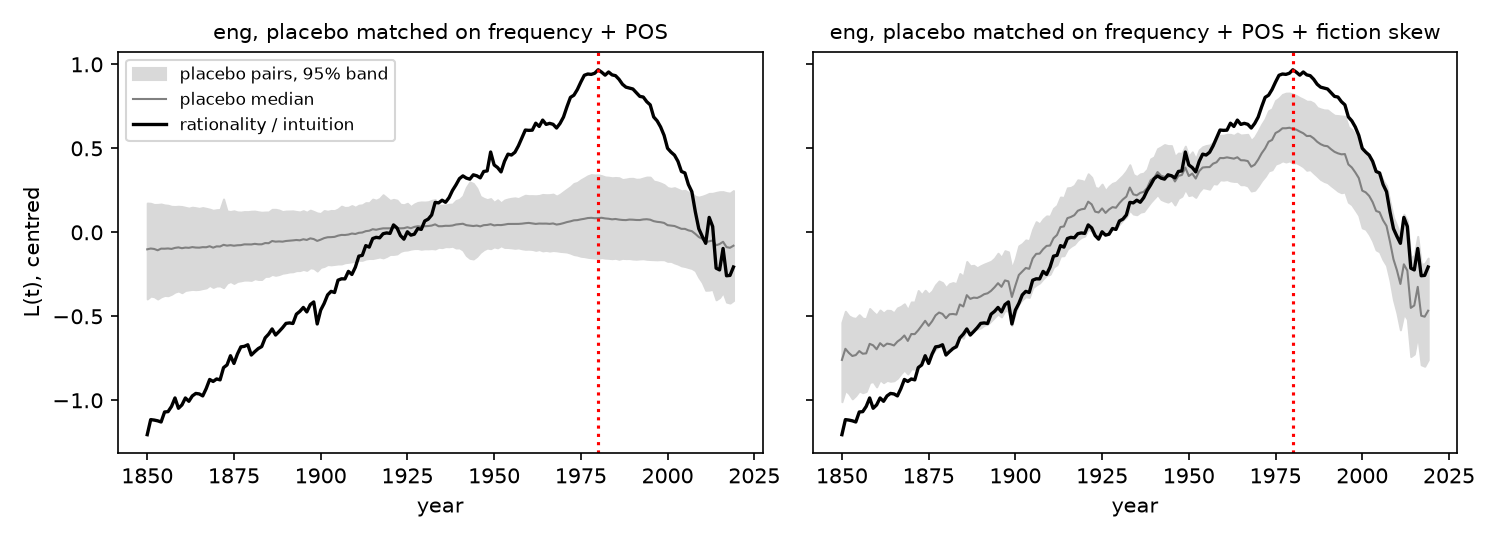
\includegraphics[width=\textwidth]{placebo_bands.png}
\caption{The log ratio $L(t)$ of the rationality and intuition words in \texttt{eng} (black, centred) and the 95\% band and median of 10,000 placebo pairs. Left: placebo words matched in frequency and part of speech. Right: matched also in fiction skew (the primary control). The dotted line is 1980.}
\label{fig:bands}
\end{figure}

\paragraph{Placebo tests.} Table~\ref{tab:main} gives all tests. Figure~\ref{fig:bands} shows the placebo bands for \texttt{eng}.

\begin{table}[h]
\centering
\small
\begin{tabular}{llrrrrrr}
\toprule
Control & Corpus & $g_{\mathrm{obs}}$ & Median $g'$ & 5\% quantile & $p$ & Reversal & $\tau^*$ in 1975--90\\
\midrule
\textbf{FPS} & \textbf{eng} & $\mathbf{-0.449}$ & $\mathbf{-0.396}$ & $\mathbf{-0.472}$ & \textbf{0.126} & \textbf{1.000} & \textbf{0.946}\\
FPS & fiction & $-0.253$ & $-0.251$ & $-0.345$ & 0.484 & 0.908 & 0.565\\
FPS & non-fiction & $-0.365$ & $-0.299$ & $-0.372$ & 0.069 & 1.000 & 0.901\\
FP & eng & $-0.449$ & $-0.057$ & $-0.173$ & 0.0001 & 0.643 & 0.227\\
FP & fiction & $-0.253$ & $-0.039$ & $-0.135$ & 0.0006 & 0.376 & 0.346\\
FP & non-fiction & $-0.365$ & $-0.041$ & $-0.136$ & 0.0001 & 0.575 & 0.210\\
Label shuffle & eng & $-0.449$ & $0.000$ & $-0.136$ & 0.0001 & 0.394 & 0.237\\
\bottomrule
\end{tabular}
\caption{Change of slope $g$ at 1980 (per decade) of the flag words and of 10,000 placebo pairs for each control. $p$ is one-sided. ``Reversal'' is the share of placebo pairs with $b>0$ and $b+g<0$. The last column is the share of pairs with the best hinge year in 1975 to 1990. The first row is the pre-registered primary test.}
\label{tab:main}
\end{table}

Against words matched only in frequency and part of speech, the turn is extreme in all three corpora ($p \le 0.0006$). It is also extreme against random splits of the flag words ($p = 0.0001$). So a test without register matching would support the specificity of the turn.

The FP placebo words do not have the register of the flag words. The mean fiction skew of $A$ is $-1.40$ and of $B$ is $+0.68$. The FP pairs have $-0.56$ and $-0.43$. The FPS pairs have $-1.34$ and $+0.62$. Against the FPS pairs, the observed turn is in the lower 13\% of the distribution ($p = 0.126$). The protocol's verdict is ``refutation of specificity''. All 10,000 FPS pairs reverse in \texttt{eng}, and 94.6\% have their best hinge year in 1975 to 1990. Inside fiction alone the observed turn is at the median of the FPS pairs ($p = 0.484$). Inside non-fiction alone $p = 0.069$.

The FPS candidates are words of the same register; they are not synonyms of the flag words. The ten nearest FPS candidates of \emph{data} are \emph{production, products, research, industry, areas, cent, systems, results, solution, temperature}. Those of \emph{soul} are \emph{horse, feeling, sort, bar, husband, police, daughter, evening, brother, arms}. The FPS pairs use 1,663 distinct pool words, and the FP pairs use 1,874.

\section{What the test can detect}\label{sec:power}
A non-rejection is informative only if the test could detect a specific effect of a useful size. The FPS null distribution of $g$ in \texttt{eng} has median $-0.396$ and standard deviation $0.047$ per decade. The observed $g$ is $0.053$ per decade more negative than the median. This excess is 12\% of $g_{\mathrm{obs}}$ (1.1 standard deviations).

To measure the sensitivity, we added an extra hinge of size $f \cdot g_{\mathrm{obs}}$ to each of the 10,000 FPS null pairs and counted the share below the null 5\% quantile. This analysis is post hoc.

\begin{center}
\begin{tabular}{lccccc}
\toprule
$f$ & 0.10 & 0.15 & 0.20 & 0.25 & 0.30\\
\midrule
Share detected & 0.252 & 0.422 & 0.609 & 0.771 & 0.885\\
\bottomrule
\end{tabular}
\end{center}

So a specific extra turn of 25\% of the observed size (about 0.11 per decade) would be detected with probability 0.77. A specific turn of 12\%, the size of the observed excess, would be detected with probability of about 0.25. The test does not exclude a specific component of that size. The protocol also reports power 1.00 for an added hinge of $d = g_{\mathrm{obs}}$ and $d = g_{\mathrm{obs}}/2$. Those numbers describe a hinge that is added on top of the register effect. They are not the power to detect the observed difference, and the table above replaces them for that purpose.

\section{How sensitive the verdict is}
\paragraph{Matching quality.} The FPS matching is not perfect. The difference of mean skew between $A'$ and $B'$ is $-1.952$ on average (standard deviation 0.042). For the flag words it is $-2.076$. Across the FPS pairs this skew gap and $g$ correlate ($r = 0.31$), so pairs with a larger gap tend to have a more negative turn. The FPS placebo therefore has a slightly weaker register contrast than the flag words, which makes a significant result easier to get. After a linear adjustment of $g$ to the observed skew gap, $p = 0.42$. This adjustment is post hoc. It moves the result further from significance.

\paragraph{Number of candidates $K$.} With the same seeds and $K = 20$ (tighter matching), the FPS $p$ is 0.219 in \texttt{eng}, 0.537 in fiction and 0.114 in non-fiction. With $K = 80$ (looser matching) it is 0.075, 0.419 and 0.050. All FP $p$-values stay at or below 0.0007. The verdict at 0.05 does not change for \texttt{eng}. The $p$-value falls when the matching becomes looser, as expected if register drives the turn. These runs are post hoc.

\paragraph{Independent implementation.} In the verification stage, a second implementation was written from the protocol alone, with other seeds and a different rule for collisions. It gave FPS $p = 0.128$ to $0.130$ in \texttt{eng} for three seeds, and FP $p \le 0.0004$.

\paragraph{The rise before 1980 (post hoc).} After the primary result, the figure showed that the flag words rise faster before 1980 than most FPS pairs. Only 0.22\% of the FPS pairs in \texttt{eng} have a slope $b$ before 1980 as large as the observed one (0.51\% in fiction, 0.20\% in non-fiction). So the rise phase is more specific to these words than the turn. This observation was not pre-registered and was not tested with a new protocol.

\section{Interpretation}
The rationality words are science-register words, and the intuition words are fiction-register words. All 10,000 FPS pairs have this register contrast, and all of them rise until about 1980 and fall after it in Google Books English. The turn of the flag words is not distinguishable from these pairs at the pre-registered threshold.

The protocol phrased the refutation outcome as ``composition is sufficient to give a turn of this size''. The data require a narrower reading. The matched turn is present inside fiction alone (91\% of the FPS pairs reverse) and inside non-fiction alone (100\% reverse). A change of the share of fiction cannot give a turn inside one of these sub-corpora. So the matched variable is a register contrast that changes inside each sub-corpus, and the growth of the fiction share is not the only mechanism. Two readings agree with this: a change of the kinds of books inside each category (for example a change of the share of scientific and professional texts, a composition effect that Pechenick et al.\ describe for the 1900s~\cite{pechenick}), and a broad change of style, such as Sun's ``colloquialization''~\cite{sun}. This study does not test either reading.

The result also agrees with a part of the source's own view. Scheffer et al.\ derive the pattern from a principal component of 5,000 words, and the flag words mark one end of it~\cite{scheffer}. A turn that all register-matched words share is consistent with a broad shift. What the result removes is the use of the flag-word ratio as evidence for a change that is specific to rationality and intuition as concepts, beyond the register in which these words are used.

\section{Limits}\label{sec:limits}
\begin{itemize}
\item The result is a non-rejection at $\alpha = 0.05$. The observed $g$ is 12\% more negative than the placebo median, and a specific extra turn of this size would be detected with probability of only about 0.25 (Section~\ref{sec:power}).
\item The matched variable, fiction skew, correlates with the meaning of the flag words: science words are rare in fiction. FPS matching therefore also removes any part of a real semantic effect that goes with register. The result says that the test finds no specificity of the turn beyond register. It does not say that meaning has no part.
\item We test one statistic: the change of slope at a fixed hinge in 1980. We do not test the acceleration around 2007, the shift from collectivistic to individualistic language, or the principal-component analysis.
\item Fiction skew is one composition variable. Other changes of composition, for example of academic or self-published books, are not matched.
\item The pool excludes words that are absent from fiction in any year and words whose lowercase form is less than half of their count. This removes some rare words and names.
\item We study English only. The source also reports Spanish and other languages.
\item All results are associations. We make no causal claim.
\end{itemize}

\begin{table}[h]
\centering
\small
\begin{tabular}{p{0.3\textwidth}p{0.62\textwidth}}
\toprule
Deviation & Effect\\
\midrule
The code removes the word ``an'' from the pool. & ``an'' has the part of speech ``other'', which no flag word has, so it cannot be drawn. It moves the pool boundary by one word. With ``an'' in the pool, the independent implementation gives $p = 0.132$ against $0.130$.\\
The extractor drops a case form with a total count (1850--2019) below 2,000, and a tagged form below 1,000. & The extracted frequencies agree with the Ngram Viewer to within 0.02\% in \texttt{eng}. In fiction, the mean ratio is 0.9989 to 1.0000; the rarest pool word has a minimum of 0.953 in one year.\\
\bottomrule
\end{tabular}
\caption{Two filters in the code that the protocol does not state. Both were found in the verification stage.}
\label{tab:dev}
\end{table}

\section{How this was checked}
\begin{itemize}
\item The script \texttt{checks/rerun.py} streams the raw data again, rebuilds the word table, clones the authors' repository for the known-answer check, runs the pre-registered analysis and the post-hoc script, and compares 419 numbers with the files \texttt{data/expected.json} and
\texttt{data/expected\_posthoc.json}. From a clean copy, the pre-registered part ran in 514~s with no mismatch.
\item The verification stage reran the pipeline from the raw data in a new clone (no mismatch), read every script against the protocol, checked the extraction against the Google Ngram Viewer, and wrote the independent implementation described above.
\item The verification stage compared the quote of the claim and the word lists with the source and the authors' notebook. Both agree.
\end{itemize}

\begin{figure}[t]
\centering
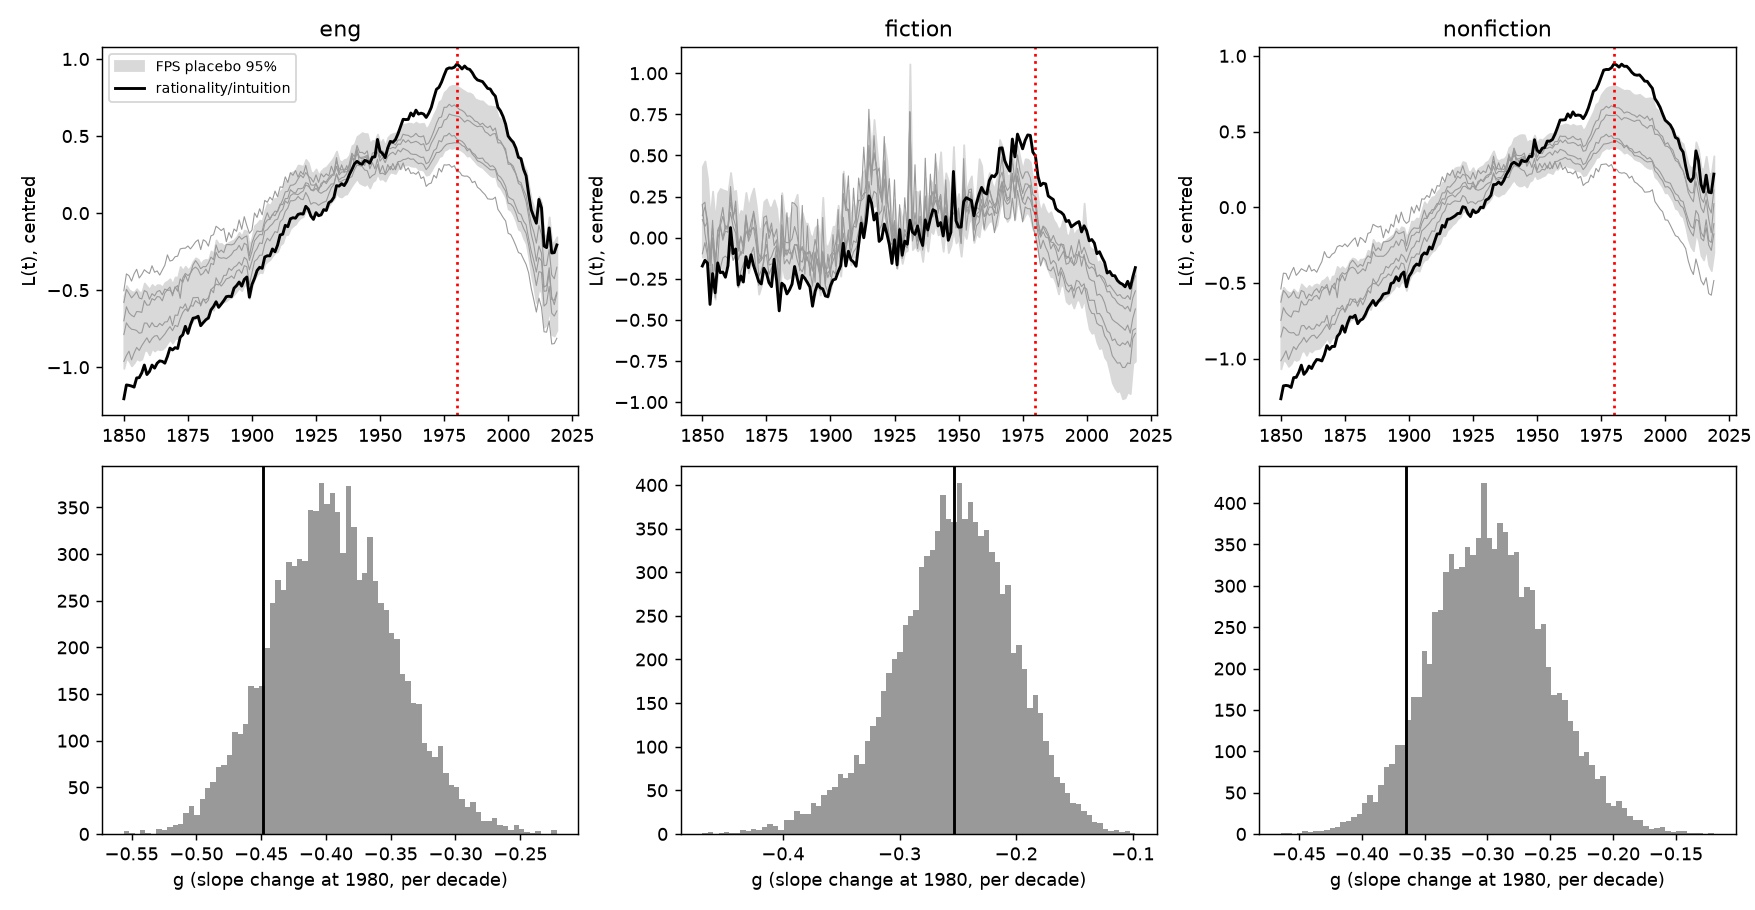
\includegraphics[width=\textwidth]{placebo.png}
\caption{Top: the observed $L(t)$ (black, centred), the 95\% band of the FPS placebo pairs (grey) and five placebo pairs, for \texttt{eng}, fiction and non-fiction. Bottom: the distribution of $g$ for the 10,000 FPS pairs; the vertical line is $g_{\mathrm{obs}}$.}
\label{fig:dist}
\end{figure}

\paragraph{Acknowledgements.} Marten Scheffer, Ingrid van de Leemput, Els Weinans and Johan Bollen published their word lists, count tables and notebooks, which made the known-answer check possible. Google published the Ngram data under CC BY 3.0.

\begin{thebibliography}{10}
\bibitem{scheffer} M. Scheffer, I. van de Leemput, E. Weinans and J. Bollen, ``The rise and fall of rationality in language,'' \emph{Proc. Natl. Acad. Sci. USA} 118(51), e2107848118 (2021). \href{https://doi.org/10.1073/pnas.2107848118}{doi:10.1073/pnas.2107848118}. Full text: PMC8713757.
\bibitem{scheffercode} M. Scheffer, I. van de Leemput, E. Weinans and J. Bollen, code and data repository \href{https://github.com/jbollen/rise_and_fall_of_rationality_in_language}{\texttt{jbollen/rise\_and\_fall\_of\_rationality\_in\_language}}, notebook \texttt{Rise\_fall\_rationality\_analysis\_Figs.ipynb}, accessed November 26, 2026.
\bibitem{ngram} Google Books Ngram Viewer, \href{https://storage.googleapis.com/books/ngrams/books/datasetsv3.html}{Exports, version 3 (20200217)}, CC BY 3.0, accessed November 26, 2026.
\bibitem{dedeo} S. DeDeo, ``Using big data to track major shifts in human cognition,'' \emph{Proc. Natl. Acad. Sci. USA} 119(4), e2121300119 (2022). \href{https://doi.org/10.1073/pnas.2121300119}{doi:10.1073/pnas.2121300119}.
\bibitem{sun} K. Sun, ``Colloquialization as a key factor in historical changes of rational and emotional words,'' \emph{Proc. Natl. Acad. Sci. USA} 119(26), e2205563119 (2022). \href{https://doi.org/10.1073/pnas.2205563119}{doi:10.1073/pnas.2205563119}.
\bibitem{reply} M. Scheffer, I. van de Leemput, E. Weinans and J. Bollen, ``Reply to Sun: Making sense of language change,'' \emph{Proc. Natl. Acad. Sci. USA} 119(26), e2206616119 (2022). \href{https://doi.org/10.1073/pnas.2206616119}{doi:10.1073/pnas.2206616119}.
\bibitem{mair} V. Mair, \href{https://languagelog.ldc.upenn.edu/nll/?p=53178}{``Language meets literature; rationality vs.\ experience; fiction vis-\`a-vis nonfiction,''} Language Log, December 30, 2021.
\bibitem{pechenick} E. A. Pechenick, C. M. Danforth and P. S. Dodds, ``Characterizing the Google Books corpus: Strong limits to inferences of socio-cultural and linguistic evolution,'' \emph{PLOS ONE} 10(10), e0137041 (2015). \href{https://doi.org/10.1371/journal.pone.0137041}{doi:10.1371/journal.pone.0137041}.
\bibitem{bollen} J. Bollen, M. ten Thij, F. Breithaupt, A. T. J. Barron, L. A. Rutter, L. Lorenzo-Luaces and M. Scheffer, ``Historical language records reveal a surge of cognitive distortions in recent decades,'' \emph{Proc. Natl. Acad. Sci. USA} 118(30), e2102061118 (2021). \href{https://doi.org/10.1073/pnas.2102061118}{doi:10.1073/pnas.2102061118}.
\bibitem{schmidt} B. Schmidt, S. T. Piantadosi and K. Mahowald, ``Uncontrolled corpus composition drives an apparent surge in cognitive distortions,'' \emph{Proc. Natl. Acad. Sci. USA} 118(45), e2115010118 (2021). \href{https://doi.org/10.1073/pnas.2115010118}{doi:10.1073/pnas.2115010118}.
\bibitem{bollenreply} J. Bollen, M. ten Thij, F. Breithaupt, A. T. J. Barron, L. A. Rutter, L. Lorenzo-Luaces and M. Scheffer, ``Reply to Schmidt et al.: A robust surge of cognitive distortions in historical language,'' \emph{Proc. Natl. Acad. Sci. USA} 118(45), e2115842118 (2021). \href{https://doi.org/10.1073/pnas.2115842118}{doi:10.1073/pnas.2115842118}.
\end{thebibliography}
\end{document}
